\chapter{\IfLanguageName{dutch}{Resultaten}{results}}%
\label{ch:resultaten}

In dit hoofdstuk worden de resultaten gepresenteerd van de uitgevoerde netwerken systeemtesten. De metingen vinden plaats in 3 verschillende netwerkomgevingen: wifi, 4G en privaat 5G. Voor elke omgeving worden gegevens verzameld over latency, jitter, packet loss, bandbreedte en througput.
De resultaten worden gegroepeerd per netwerktype en gevisualiseerd met behulp van grafieken en tabellen. Naast objectieve meetwaarden wordt ook de functionele impact op de communicatie met HVAC- en verlichtingssimulaties besproken.


\section{Netwerkprestaties}

De netwerkprestaties worden vergeleken op basis van:

\begin{itemize}
    \item \textbf{Gemiddelde latency} (ms): de tijd tussen het verzenden en ontvangen van datapakketten;
    \item \textbf{Jitter} (ms): de variatie in vertragingstijd tussen opeenvolgende pakketten;
    \item \textbf{Packet loss} (\%): het percentage datapakketten dat verloren gaat tijdens verzending;
    \item \textbf{Bandbreedte} (Mbit/s): de gemeten download- en uploadsnelheden.
\end{itemize}

\subsection{Latency}
Latency is de tijd die een datapakket nodig heeft om van verzender naar ontvanger te reizen. In toepassingen zoals lichtsturing of HVAC-automatisering is een lage en stabiele latency belangrijk om opdrachten snel en voorspelbaar uit te voeren.

De resultaten zijn samengevat in Tabel \ref{tab:latency} en figuur \ref{fig:latency}.
\begin{table}[]
    \caption{Resultaten van de ping-test} \label{tab:latency}
        \begin{tabular}{l l l l}
            \cline{2-4}
            & \textbf{RTT avg (ms)} & \textbf{RTT min (ms)} & \textbf{RTT max (ms)} \\ \hline
            \multicolumn{1}{l}{\textbf{wifi}} & 13,27          & 12,85          & 18,05           \\ \hline
            \multicolumn{1}{l}{\textbf{4G}}   & 18,17         & 15,66           & 37,05           \\ \hline            
            \multicolumn{1}{l}{\textbf{5G}}   & 26,30           & 10,85            & 230,92         \\ \hline
        \end{tabular}
        
        %\caption*{Note. uitleg bij tabel}
    
\end{table}

\begin{figure}
    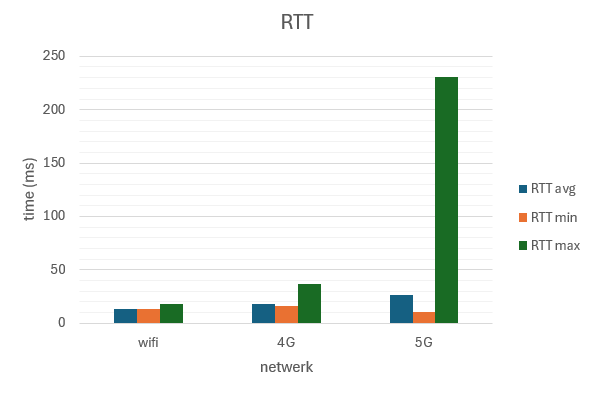
\includegraphics[width=0.8\textwidth]{../graphics/RTT_grafiek.png}
    \caption[Grafiek van de gemiddelde resultaten van de ping test]{\label{fig:latency}Grafiek van de gemiddelde resultaten van de ping test}
\end{figure}
\subsubsection{Analyse}
\begin{itemize}
    \item wifi vertoont de laagste gemiddelde latency (13,27 ms). Dit bevestigt de stabiliteit van het lokale draadloze netwerk in een gecontroleerde binnenomgeving zonder externe overbelasting.
    \item 4G toont een iets hogere gemiddelde latency (18,17 ms), wat in lijn ligt met de verwachte vertraging van een mobiel netwerk door de routing via het publieke netwerk van de provider.
    \item 5G levert tegenstrijdige resultaten: de minimum RTT (10,85 ms) is het laagst voor 5G wat wijst op het potentieel van de technologie voor lage latency. Tegelijkertijd is de gemiddelde RTT aanzienlijk hoger (26,30 ms) door RTT-waarden die pieken tot 230,92 ms. Dit kan wijzen op instabiliteit of fluctuaties tijdens de test, mogelijk door beperkte dekking, interferentie of routerproblemen in het privaat 5G-netwerk.
\end{itemize}
Hoewel 5G in theorie de laagste latency kan bieden, werd bij deze metingen minder stabiele resultaten waargenomen. Dit kan veroorzaakt zijn door onvoldoende configuratie van het privaat 5G-netwerk, een lage signaalsterkte of routingproblemen bij het verzenden van dataverkeer naar het internet.

\subsubsection{Aanbeveling}
Aangezien deze test werd uitgevoerd naar een extern IP-adres (8.8.8.8), is het resultaat niet volledig representatief voor de prestaties van het interne netwerksegment.
Verkeer naar het internet ondergaat additionele vertragingen door publieke netwerkrouting, congestie, of provider Service Level Agreements. Daarom wordt aanbevolen om latency-testen uit te voeren naar een lokaal IP-adres binnen het testnetwerk. Hierdoor worden enkel de prestaties van het interne netwerkpad gemeten. Dit is relevanter voor de eindtoepassing van HVAC- en lichtsturing, die binnen het campusnetwerk plaatsvinden. Een aangepaste testopstelling met: \textbf{ping -c 250 [lokaal-IP]} zal vermoedelijk beter inzicht bieden in de betrouwbaarheid en reactietijd van de onderzochte netwerken, zonder verstoring door externe internetrouting.


\subsection{Jitter}
Jitter is een maat voor de variabiliteit in de vertragingstijd tussen verzenden en ontvangen van opeenvolgende datapakketten. In real-time toepassingen zoals HVAC-sturing of lichtregeling zou een hoge jitter-waarde kunnen leiden tot inconsistente werking zoals vertraagde of incorrect uitgevoerde commando’s.

De UDP-test werd uitgevoerd met iperf3 op drie verschillende snelheden (1, 5 en 50 Mbit/s), telkens gedurende 120 seconden. De resultaten zijn samengevat in Tabel \ref{tab:jitter} en figuur \ref{fig:jitter}.

\begin{table}[]
    \caption{Gemeten jitter (in ms) bij verschillende UDP-bandbreedtes}
    \begin{tabular}{l l l l}
        \cline{2-4}
        & \textbf{1 Mbits/s} & \textbf{5 Mbits/s} & \textbf{50 Mbits/s} \\ \hline
        \multicolumn{1}{l}{\textbf{wifi}} & 0,799              & 0,620                 & 0,158               \\ \hline
        \multicolumn{1}{l}{\textbf{4G}}   & 0,313                & 0,151                & 0,189               \\ \hline
        \multicolumn{1}{l}{\textbf{5G}}   & 0,380               & 0,171                & 0,198               \\ \hline
    \end{tabular}
    
    \label{tab:jitter}
\end{table}
\begin{figure}

    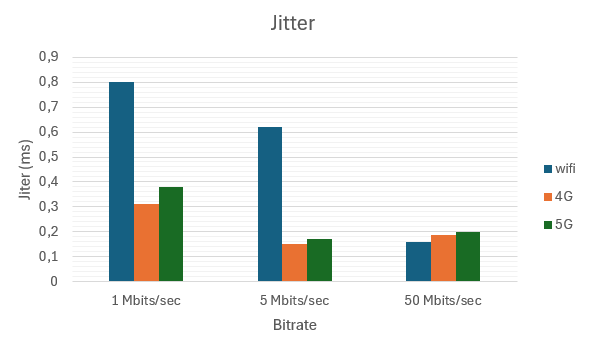
\includegraphics[width=0.8\textwidth]{../graphics/Jitter_grafiek.png}
    \caption[Grafiek van de gemiddelde resultaten van de iperf3 TCP test]{\label{fig:jitter}Grafiek van de gemiddelde resultaten van de iperf3 TCP test}
\end{figure}
\subsubsection{Analyse}
Bij een lage datasnelheid van 1 Mbit/s vertoont wifi de hoogste jitter (0,799 ms), wat mogelijk wijst op instabiliteit of interferentie in het lokale draadloze netwerk. 4G en 5G hebben bij 1Mbit/s een lagere vertragingstijd, met respectievelijk 0,313 ms en 0,380 ms. Op 5 Mbit/s zien we een duidelijke afname van jitter over alle netwerken. Vooral bij 4G is dit opmerkelijk: slechts 0,151 ms, wat wijst op een stabiele verbinding onder matige belasting. Bij hogere belasting (50 Mbit/s) convergeert de jitterwaarde voor alle netwerken naar een gelijkaardig niveau (tussen 0,158 en 0,198 ms), wat duidt op een goede afhandeling van het dataverkeer, zelfs bij intensieve communicatie. 

\subsubsection{Aanbeveling }
Voor toepassingen met tijdkritische communicatie zoals gebouwautomatisering is een lage jitter cruciaal. Op basis van deze resultaten blijkt dat alle netwerken bij hogere bandbreedtes redelijk stabiel presteren. 4G biedt in de gehele test de beste balans tussen lage jitter en betrouwbaarheid bij lagere snelheden. Indien de prioriteit ligt op minimale variatie in responstijden, bijvoorbeeld voor regelkringen of kritieke commando’s, is het aanbevolen om 4G of 5G boven wifi te verkiezen. Zeker in storingsgevoelige omgevingen kan wifi minder voorspelbaar zijn.


\subsection{Packet loss}

\subsubsection{Analyse}
Packet loss is een belangrijke parameter bij het evalueren van de betrouwbaarheid van netwerkverbindingen. In toepassingen zoals HVAC- en verlichtingssturing, waar ieder signaal telt, kan verlies van datapakketten leiden tot gemiste of vertraagde commando’s, wat de functionaliteit en veiligheid van het systeem kan ondermijnen.

Om packet loss te evalueren zijn twee afzonderlijke testen uitgevoerd:
\begin{itemize}
    \item Een \textbf{ping-test} met 250 opeenvolgende pakketten naar \texttt{8.8.8.8}.
    \item Een \textbf{UDP-throughputtest} met \texttt{iperf3}, waarbij gedurende 120 seconden continu UDP-verkeer werd gegenereerd.
\end{itemize}

Bij de ping-test blijkt uit de resultaten dat er geen pakket verlies is  bij alle drie de geteste netwerken. De succesratio bedraagt in elke testsetting 100\%, wat wijst op een betrouwbare datapad voor kleine, periodieke datapakketten. Dit is vergelijkbaar met wat gebruikt wordt bij polling- of statussignalen.
Ook bij de UDP-test met iperf3 zijn er geen meldingen van dataverlies. De iperf3-uitvoer toont een packet loss van 0\% voor alle netwerken. Zelfs bij hogere verzendsnelheden (rond 94 Mbit/s over 120 seconden) wordt het volledige volume van verzonden data correct ontvangen. Dit geeft aan dat de netwerken, ondanks hun verschillen in latency en jitter (zie punt 5.1.1 en 5.1.2), in staat zijn om stabiele datapaden te leveren zonder verlies, zelfs bij een relatief hoge netwerkbelasting.


\subsubsection{Aanbevelingen}
Deze resultaten bevestigen dat in de huidige testopstelling, de onderzochte netwerken in staat zijn om dataverlies te vermijden. Dit is essentieel is voor een correcte en voorspelbare werking van automatiseringssystemen in gebouwen.
Maar het is belangrijk om bij uitbreiding de parameter packet loss ook onder realistischere omstandigheden (zoals roaming, zwakker signaal of congestie) verder te testen als migratie naar mobiele netwerken overwogen wordt voor de sturing van kritieke gebouweninfrastructuur.



\subsection{Bandbreedte en netwerkcapaciteit}
Om de prestaties van elk netwerktype te evalueren onder continue belasting, wordt een TCP throughput-test uitgevoerd met behulp van \texttt{iperf3}. Tijdens deze test wordt gedurende 120 seconden data van een client naar een server verzonden. Twee belangrijke prestatie-indicatoren worden hierbij gemeten:

\begin{itemize}
    \item \textbf{Bitrate (Mbit/s)}: de gemiddelde hoeveelheid data die per seconde succesvol wordt overgedragen;
    \item \textbf{Congestion Window (cwnd)}: de maximale hoeveelheid data (in bytes) die op een bepaald moment zonder bevestiging mag worden verzonden. Hoe groter dit venster, hoe efficiënter de verbinding.
\end{itemize}

De meetresultaten staan in Tabel \ref{tab:bandbreedte}.

\begin{table}[]
    \caption{Gemeten gemiddelde bitrate en congestion window per netwerk (iperf3 TCP-test)}
    \begin{tabular}{l l l}
        \cline{2-3}
        & \textbf{Bitrate (Mbits/s} & \textbf{Cwnd (Bytes)} \\ \hline
        \multicolumn{1}{l}{\textbf{wifi}} & 94,28                    & 412,76              \\ \hline
        \multicolumn{1}{l}{\textbf{4G}}   & 94,23                      & 421,37              \\ \hline
        \multicolumn{1}{l}{\textbf{5G}}   & 931,16                    & 655,37              \\ \hline
    \end{tabular}
    
    \label{tab:bandbreedte}
\end{table}

\subsubsection{Analyse}
De resultaten tonen dat wifi en 4G vergelijkbare bitrates hebben, beide net boven de 94 Mbit/s. Dit suggereert dat de limiet hier niet in het netwerk zelf ligt, maar eerder aan de zijde van de testapparatuur of netwerkinstellingen (zoals 100 Mbit/s ethernetpoort of NAT-overhead).
5G presteert daarentegen aanzienlijk beter, met een gemiddelde bitrate van meer dan 931 Mbit/s. Dit is bijna tien keer hoger dan bij de andere netwerken. Dit bevestigt de hoge doorvoercapaciteit van een standalone 5G-infrastructuur en toont aan dat dit netwerk veel geschikter is voor toepassingen die grote hoeveelheden datauitwisseling vereisen.
Het congestion window (cwnd) ondersteunt deze conclusie: bij 5G is dit beduidend groter (655.369 bytes), wat aangeeft dat de zender het netwerk als stabiel en betrouwbaar ervaart. Dit laat grotere hoeveelheden data toe per verzendcyclus, wat bijdraagt aan hogere efficiëntie en minder vertraging.

\subsubsection{Aanbeveling}
Hoewel de aansturing van HVAC- en verlichtingssystemen op zich geen hoge bandbreedte vereist, biedt het 5G-netwerk voordelen met het oog op toekomstige uitbreiding. Dit kan gaan over real-time monitoring, integratie met slimme sensoren of het centraliseren van gebouwbeheer via cloudgebaseerde dashboards.
Voor eenvoudige commando’s of basisautomatisering blijven 4G en wifi voldoende. Op basis van de testen van de prestaties van het 5G netwerk zal hier wel de voorkeur aan kunnen gegeven worden voor schaalbaarheid, betrouwbaarheid en datacapaciteit. Dit zijn belangrijke criteria om te bekijken bij o.a. het langetermijnbeleid van het gebouwenbeheersysteem van HOGENT.



\newpage
\section{Functionele testen}

Deze sectie onderzoekt of de netwerken geschikt zijn voor automatisering van operationele taken zoals aan/uit schakelen van verlichting of HTTP-verkeer via Node-RED. De nadruk ligt hierbij op reactietijd en betrouwbaarheid.

\subsection{Verlichtingstest}

In deze test wordt de reactietijd gemeten tussen het versturen van een commando via het netwerk en het schakelen van een slimme lamp. Dit type scenario is representatief voor veelgebruikte toepassingen binnen domotica en gebouwbeheer, zoals het automatisch activeren van verlichting op basis van sensoren of tijdsinstellingen. De resultaten staan in Tabel \ref{tab:licht}.

\begin{table}[]
    \caption{Resultaten lichtschakelingstest}
    \begin{tabular}{l l l}
        \cline{2-3}
        & \textbf{Gem reactiesnelheid (ms)} & \textbf{succes rate} \\ \hline
        \multicolumn{1}{l}{\textbf{wifi}} & 224,16                            & 100\%                \\ \hline
        \multicolumn{1}{l}{\textbf{4G}}   & 113,80                             & 100\%                \\ \hline
        \multicolumn{1}{l}{\textbf{5G}}   & 90,63                             & 100\%                \\ \hline
    \end{tabular}
    \label{tab:licht}
\end{table}

\subsubsection{Analyse}
Tijdens de test werd het schakelsignaal via drie verschillende netwerken verzonden: wifi, 4G en 5G. Alle netwerken slaagden erin om het licht betrouwbaar aan en uit te schakelen, zonder dat er signalen verloren gingen of vertraagd aankwamen tot het punt van falen. De gemiddelde reactietijden lieten echter duidelijke verschillen zien:
\begin{itemize}
    \item \textbf{wifi} vertoonde een merkbaar hogere reactietijd, hoewel deze nog steeds toelaatbaar was voor de meeste toepassingen.
    \item \textbf{4G} presteerde iets trager, maar bleef binnen een acceptabele marge voor real-time toepassingen.
    \item \textbf{5G} behaalde de laagste gemiddelde reactietijd (\textit{90,63} ms), wat wijst op een zeer snelle signaalverwerking.
\end{itemize}

Deze resultaten suggereren dat mobiele netwerken, en in het bijzonder 5G, bijzonder goed geschikt zijn voor tijdgevoelige IoT-acties waarbij directe feedback cruciaal is.

\subsubsection{Aanbevelingen}
Op basis van de meetresultaten kan worden geconcludeerd dat zowel 4G als 5G goede opties vormen voor automatiseringsscenario’s waar snelheid en betrouwbaarheid essentieel zijn. Vooral in toepassingen waarbij de respons van systemen direct zichtbaar of merkbaar moet zijn voor gebruikers (zoals verlichting of alarmering), bieden deze netwerken een technisch voordeel.

Toch is het aanbevolen om rekening te houden met contextuele factoren:
\begin{itemize}
    \item In een sterk belast wifi netwerk (bijv. gedeeld in een kantooromgeving), kunnen vertragingen oplopen. In dat geval bieden mobiele netwerken een betrouwbaarder alternatief.
    \item Voor toepassingen waarbij ultra-lage latentie vereist is (zoals interactie met bewegingssensoren of real-time synchronisatie), verdient 5G de voorkeur.
    \item Bij het ontwerpen van automatiseringssystemen moet ook de variabiliteit in netwerkprestaties (bijvoorbeeld tijdens piekuren) worden meegewogen.
\end{itemize}

Het verdient aanbeveling om bij grootschalige implementatie van verlichtings- of actuatorsystemen netwerkkeuze te baseren op lokale performance tests en gebruiksprofielen.

\subsection{HTTP-verkeer (Node-RED test)}

Deze test evalueert de prestaties van HTTP-verkeer, zoals vaak gebruikt in moderne IoT-platformen. Via het Node-RED automatiseringsplatform werd elke vijf seconden een HTTP-aanvraag verzonden naar een lokaal endpoint. Daarbij werden zowel download- als uploadcapaciteit gemeten, evenals de totale verwerkingstijd van de aanvragen.

\begin{table}[h]
    \caption{Gemiddelde doorvoersnelheden van HTTP-verkeer in Node-RED test}
    \label{tab:nodered}
    \begin{tabular}{l l l l}
        \cline{2-4}
        & \textbf{Dload (bytes/s)} & \textbf{Uload (bytes/s)} & \textbf{Current speed (bytes/s)} \\ \hline
        \multicolumn{1}{l}{\textbf{wifi}}       & 1338,49                     & 1003,72                    & 2507,29                             \\ \hline       
        \multicolumn{1}{l}{\textbf{4G}} & 3870,21                     & 2902,56                    & 8026,70                             \\ \hline
        \multicolumn{1}{l}{\textbf{5G}} & 2546,55                     & 1909,75                    & 5077,83                             \\ \hline
    \end{tabular}
    
\end{table}
\begin{figure}
    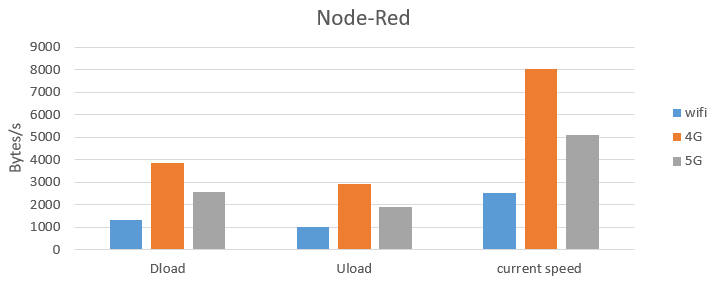
\includegraphics[width=0.8\textwidth]{../graphics/Node-red_grafiek.png}
    \caption[Grafiek van de Node-Red test met de gemiddelde waarden per netwerk]{\label{fig:noderedgem}Grafiek van de Node-Red test met de gemiddelde waarden per netwerk}
\end{figure}
\begin{figure}

    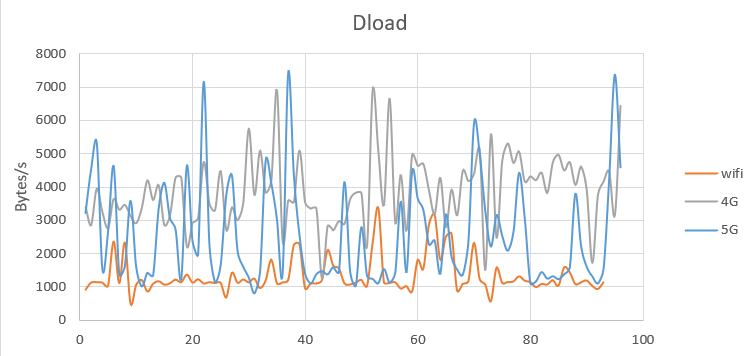
\includegraphics[width=0.8\textwidth]{../graphics/node-red_dload_grafiek.png}
    \caption[Spreidingsgrafiek van de Download waarden van de Node-Red test]{\label{fig:nodereddload}Spreidingsgrafiek van de Download waarden van de Node-Red test}
\end{figure}
\begin{figure}

    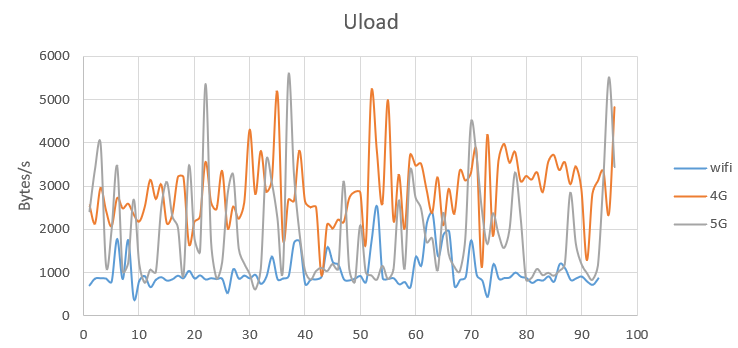
\includegraphics[width=0.8\textwidth]{../graphics/node-red_uload_grafiek.png}
    \caption[Spreidingsgrafiek van de Upload waarden van de Node-Red test]{\label{fig:nodereduload}Spreidingsgrafiek van de Upload waarden van de Node-Red test}
\end{figure}
\begin{figure}

    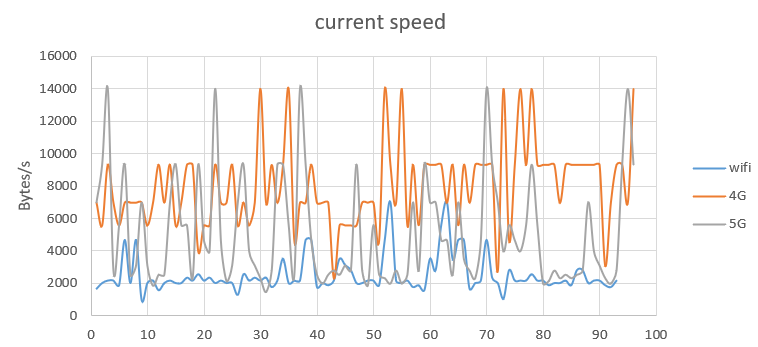
\includegraphics[width=0.8\textwidth]{../graphics/node-red_currentspeed_grafiek.png}
    \caption[Spreidingsgrafiek van de Current speed waarden van de Node-Red test]{\label{fig:noderedcs}Spreidingsgrafiek van de Current speed waarden van de Node-Red test}
\end{figure}
\subsubsection{Analyse}

De testresultaten (zie tabel \ref{tab:nodered} en figuren \ref{fig:noderedgem}, \ref{fig:nodereddload}, \ref{fig:nodereduload}, \ref{fig:noderedcs}) toonden aan dat:
\begin{itemize}
    \item \textbf{wifi} had de laagste prestaties, met enkele pieken in vertraging, mogelijk veroorzaakt door lokale interferentie of bandbreedteverdeling met andere apparaten.
    \item \textbf{4G} de hoogste gemiddelde doorvoersnelheid behaalde, met consistente prestaties over de testduur.
    \item \textbf{5G} volgde dicht daarachter, maar vertoonde iets meer variatie in snelheid, vermoedelijk door netwerkoptimalisaties of achtergrondprocessen.
    
\end{itemize}

Ondanks deze verschillen zijn alle netwerken in staat gebleken om HTTP-verkeer vlot te verwerken. De wachttijden bleven in alle gevallen ruim onder de grens die problematisch zou zijn voor typische IoT-communicatie zoals REST-aanroepen of statusupdates. Dit bevestigt de geschiktheid van elk getest netwerk voor scenario’s zoals monitoring, logging en eenvoudige afstandsbediening.

\subsubsection{Aanbevelingen}
Voor toepassingen waarin periodieke communicatie centraal staat, zoals bij statusmonitoring, gegevenslogboekregistratie of eenvoudige commando-uitwisseling, zijn alle drie netwerken voldoende performant. Toch kunnen sommige netwerken voordeliger zijn afhankelijk van de specifieke vereisten en gebruiksomstandigheden:

\begin{itemize}
    \item \textbf{wifi} blijft relevant binnen gecontroleerde, vaste omgevingen (zoals binnen gebouwen) waar bandbreedte en stabiliteit verzekerd zijn, maar moet met voorzichtigheid gebruikt worden bij gedeelde netwerken.
    \item \textbf{4G} biedt een uitstekende combinatie van snelheid, bereik en stabiliteit, en kan daarom een goede keuze zijn voor toepassingen buiten stedelijke gebieden of bij mobiele installaties.
    \item \textbf{5G} is technisch krachtig, maar vereist goede dekking om zijn volledige potentieel te benutten. In omgevingen met gegarandeerde 5G-dekking is het de beste keuze voor toekomstbestendige installaties.
    
\end{itemize}

Het wordt aanbevolen om bij de selectie van een netwerk niet enkel naar snelheid te kijken, maar ook naar betrouwbaarheid, stabiliteit over tijd, en het vermogen om met piekverkeer om te gaan. In kritieke toepassingen is een redundante netwerkopstelling (bijv. met fallback naar 4G) het overwegen waard.





